\documentclass[11pt]{article}

\usepackage[a4paper,margin=2.3cm]{geometry}
\usepackage[T1]{fontenc}
\usepackage[utf8]{inputenc}
\usepackage{lmodern}
\usepackage{microtype}
\usepackage{amsmath,amssymb}
\usepackage{graphicx}
\usepackage{array}
\usepackage{xcolor}
\usepackage{enumitem}
\setlist{itemsep=2pt,topsep=4pt}
\usepackage{lineno}
\usepackage{listings}
\lstset{basicstyle=\ttfamily\small, columns=fullflexible, keepspaces=true,
  frame=single, rulecolor=\color{black!25}, backgroundcolor=\color{black!3},
  xleftmargin=1.5em, xrightmargin=1.5em, aboveskip=6pt, belowskip=6pt}
\lstdefinestyle{cfg}{basicstyle=\ttfamily\footnotesize}
\usepackage{authblk}
\usepackage[numbers,sort&compress]{natbib}
\usepackage{xr-hyper}
\externaldocument[S-]{../supplementary/supplementary}
\usepackage[colorlinks=true,linkcolor=teal,citecolor=teal,urlcolor=teal]{hyperref}

\title{\texttt{Phyloom}: a flexible and extensible framework for simulating phylogenetic trees and networks}
\author[1,2]{Gabriele Marino}
\author[1,2]{Daniele Silvestro}
\author[1,2]{Tanja Stadler}
\affil[1]{Department of Biosystems Science and Engineering, ETH Zurich, Basel, Switzerland}
\affil[2]{SIB Swiss Institute of Bioinformatics, Basel, Switzerland}
\date{}

\begin{document}
\maketitle
\linenumbers

\begin{abstract}
  \noindent\textbf{Summary:} Simulated phylogenies underpin the validation of
  phylogenetic and phylodynamic inference methods, simulation-based hypothesis
  testing, and the training of likelihood-free estimators. Existing simulators
  cover many established models collectively, but each offers only a fixed menu
  of features on its own. Implementing even a slight tweak to a model---a common
  necessity when developing new methods---often forces users to write a
  simulator from scratch. We present \texttt{phyloom}, a Python framework in
  which simulators are instead assembled from interchangeable parts: event rules
  on lineage primitives, generic time- and model-dependent rate functions,
  scheduled actions, and user-defined stopping and acceptance criteria.
  Configured entirely through YAML without code, \texttt{phyloom} unifies
  standard phylogenetic and phylodynamic model families within a single
  tool. Priors, rejection sampling, and parallel execution turn dataset
  generation into a single command. Plugins can add custom
  models---including non-Markovian dynamics with individual-level
  memory---in just a few dozen to a few hundred lines of code.

  \medskip\noindent\textbf{Availability and implementation:} \texttt{phyloom} is
  implemented in Python ($\geq$3.10), released under the MIT license, and
  available from PyPI (\texttt{pip install phyloom}) and
  \url{https://github.com/gabriele-marino/phyloom}. Documentation and tutorials
  are at \url{https://gabriele-marino.github.io/phyloom/home}.

  \medskip\noindent\textbf{Contact:} \href{mailto:gmarino@ethz.ch}{gmarino@ethz.ch}
\end{abstract}

\section{Introduction}

Phylogenetic trees and networks hold the evolutionary trace of how species,
populations, or pathogen lineages have diversified. Phylodynamic methods
use these phylogenies to quantify the processes that created them, including
transmission, recovery, diversification, and population size changes over
time~\citep{stadler2024decoding}.
Simulating phylogenies using explicit stochastic models serves as a
core tool for developing phylodynamic models: it validates inference
software through simulation-based
calibration~\citep{talts2018sbc, mendes2025validate},
underpins posterior-predictive model
assessment~\citep{bollback2002adequacy, duchene2019phylodynadequacy}
and identifiability studies~\citep{louca2021identifiability}, and,
most recently, supplies the training data of likelihood-free
estimators~\citep{voznica2022phylodeep, lambert2023deep}.

A vast range of simulation tools exist to for a variety of different
tree generating models:
\texttt{TreeSim}~\citep{stadler2011treesim} for birth--death models,
\texttt{nosoi}~\citep{lequime2020nosoi} for epidemic transmission,
\texttt{msprime}~\citep{baumdicker2022msprime} for coalescent genealogies, and
\texttt{SiPhyNetwork}~\citep{justison2023siphynetwork} for
birth--death--hybridization networks. Nonetheless, each has its own interface and
configuration language, and a fixed menu of hardcoded models rather than
reusable primitives. Combining features across tools, such as reticulation with
a structured, time-varying epidemic, or adding a custom process thus means
compromising on the model, editing a library's core code, or writing a new
simulator, often from scratch. Even \texttt{ReMASTER}~\citep{vaughan2024remaster},
a very flexible phylodynamic simulator, is restricted to reactions with
mass-action propensities and piecewise-constant rates, i.e.\ to processes that
obey a time-inhomogeneous chemical master equation: it cannot express a rate
that depends on population size in any other functional form, or a lineage that
carries individual memory.

Here we present \texttt{phyloom}, which builds simulations from small,
interchangeable components---event rules, hazards, rate multipliers, and
scheduled actions---rather than from a fixed catalog of models. Any event can
have an arbitrary time-dependent hazard and a state-dependent rate multiplier,
with custom stopping and acceptance criteria, so that birth--death processes,
coalescent genealogies, and compartmental epidemics share a single framework.
Custom logic, such as non-Markovian dynamics with per-lineage memory, is added
through plugins without modifying the core simulator.

\section{A generic event-driven engine}
\label{sec:engine}

\texttt{Phyloom} separates what a stochastic event does from when it
happens. A model holds a system state $X(t)$ (the current lineages, their
discrete state labels, and any auxiliary quantities such as host pools) and a
list of events. Each event pairs an event rule with a hazard. The
rule counts the number $c$ of opportunities to fire in the current state (for
example, the number of current lineages in a given state, or the number of
lineage pairs that can coalesce or hybridize) and, when selected, applies one
opportunity drawn uniformly at random. The hazard $\lambda(t)$ gives the
per-opportunity rate as a function of time, and an optional
rate multiplier $m(X)$ scales it by any function of the current system
state. \texttt{Phyloom} also supports scheduled actions, which are arbitrary
operations executed at fixed times, such as sampling each lineage with
a fixed probability, or introducing new lineages. Furthermore, actions
and events can dynamically trigger or schedule additional actions and
events during a running simulation, providing the flexibility to model
complex scenarios---such as a runtime mutation event creating a new
lineage class characterized by an increased transmission rate.

For every transition, the scheduler draws $E \sim \mathrm{Exp}(1)$ for
each stochastic event and solves
\begin{equation}
  c\, m(X) \int_{t_0}^{t} \lambda(s)\,\mathrm{d}s = E
  \label{eq:firing}
\end{equation}
for the proposed firing time $t$ by inverting the cumulative hazard. The clock
then advances to the earliest proposal, the earliest deterministic
scheduled action, or a user-defined time limit, whichever comes first.
Because the system state is constant between transitions, this is an exact
stochastic simulation algorithm: with constant rates it reduces to the
Next Reaction Algorithm~\citep{gillespie1977exact, Gibson2000}, and
with time-varying hazards it simulates the corresponding non-homogeneous
process exactly~\citep{anderson2007modified}.

\section{Flexible and extensible dataset generation}
\label{sec:dataset}

\begin{figure}[ht]
  \centering
  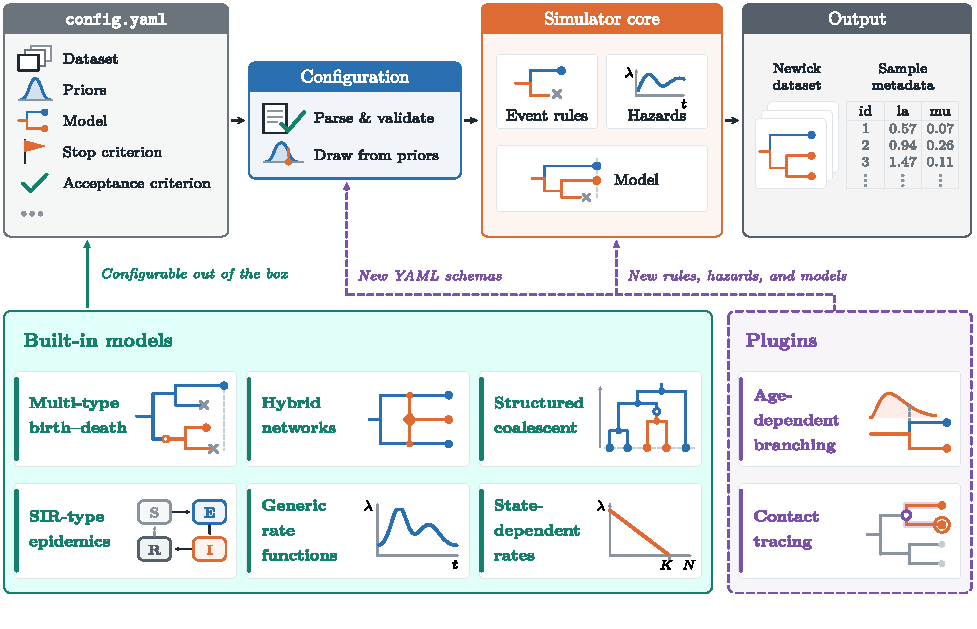
\includegraphics[width=\linewidth]{figures/pipeline.pdf}
  \caption{\texttt{Phyloom}'s pipeline, from configuration to dataset. A single YAML
    file defines how many simulations to run, the model as a list of event rules
    and their hazards, the priors on the model parameters,
    when a simulation trial ends and whether it is kept. The configuration layer
    validates it and materializes one model per simulation trial by drawing from the
    priors; the simulator core runs that model under a common scheduler.
    The dataset pairs each output phylogeny (annotated
    trees or networks in extended Newick format) with metadata records holding
    the drawn parameter values. \texttt{Phyloom} offers a library of built-in models,
    and users can add new ones as plugins.
  }
  \label{fig:pipeline}
\end{figure}

In \texttt{phyloom}, a configuration file specifies a model, a context of
per-sample parameter priors, and stopping and acceptance rules. For every
sample, the configuration layer validates this specification and materializes
the context into a concrete model, which the simulator core advances with the
engine described above (\S\ref{sec:engine}; Fig.~\ref{fig:pipeline}). A
complete configuration is short: the file below generates 1000 trees of 100
sampled tips each under a constant-rate birth--death process, drawing the
birth, death, and sampling rates anew from uniform priors for every tree:
\begin{lstlisting}[style=cfg]
output_dir: outputs/BD-minimal
n_samples: {train: 1000}
seed: 42
context:
  la: {type: uniform, low: 0.5, high: 1.5}
  mu: {type: uniform, low: 0.0, high: 0.4}
  psi: {type: uniform, low: 0.05, high: 0.3}
model:
  spec: bdsh
  init_state: I
  events:
    - rule: {spec: birth}
      hazard: {spec: constant, rate: la}
    - rule: {spec: death}
      hazard: {spec: constant, rate: mu}
    - rule: {spec: sampling, removal: true}
      hazard: {spec: constant, rate: psi}
stop_criterion: model.count_sampled_lineages() == 100
acceptance_criterion: model.count_current_lineages() > 0
output_hooks:
  - model.history(model.get_sampled_lineages()).dump(output_dir / "tree.nwk")
\end{lstlisting}

Here \texttt{n\_samples} specifies how many simulations to run for each split,
i.e.\ partition of the dataset such as training, validation, or test (here only
\texttt{train}). The runner writes each split to its own directory under
\texttt{output\_dir}, with one folder per simulation holding the files produced
by the output hooks (here \texttt{train/data/1/tree.nwk},
\texttt{train/data/2/tree.nwk}, \ldots) and a single
\texttt{train/metadata.csv}. Each \texttt{tree.nwk} is the simulated phylogeny in Newick format,
with nodes labelled by identifier and lineage state (extended Newick for
networks), and \texttt{metadata.csv} has one row per simulation with the drawn
values of \texttt{la}, \texttt{mu}, and \texttt{psi}. Phylogenies and the
parameters that generated them are thus paired by construction, as needed for
simulation-based calibration and likelihood-free
estimators~\citep{voznica2022phylodeep}.

\texttt{Phyloom} provides standard phylogenetic models out of the box, many
given as complete worked configurations in the Supplementary Material:
constant-rate~\citep{stadler2010sampling}, skyline~\citep{stadler2013bdsky},
multi-type~\citep{kuhnert2016bdmm}, and
state-dependent~\citep{maddison2007bisse} birth--death models
(Supplementary Section~\ref{S-sec:bdsh-models}), with hybridization
networks~\citep{justison2023siphynetwork} (Supplementary
Section~\ref{S-sec:bdsh}); structured~\citep{notohara1990coalescent} and
serially sampled~\citep{drummond2002serial}
coalescents~\citep{kingman1982coalescent} with arbitrary effective
population-size trajectories~\citep{griffiths1994varying} (Supplementary
Section~\ref{S-sec:coalescent-models}); and density-dependent
compartmental epidemics~\citep{kermack1927contribution} (Supplementary
Section~\ref{S-sec:epidemic-models}). In all of them, a hazard may be any expression of
time (Supplementary Section~\ref{S-sec:seasonal-bd}), and any rate may be scaled
by any function of the current state, such as clade diversity or prevalence
(Supplementary Section~\ref{S-sec:diversity-dependent}).

\texttt{Phyloom} also supports optional post-commands, which execute after the
output hooks for each sample. This allows external simulators of sequence or
trait evolution to be integrated seamlessly into the pipeline. For example,
simulating an alignment along every tree requires only a single post-command
passing the tree to \texttt{AliSim}~\citep{lytrong2022alisim}
(Supplementary Section~\ref{S-sec:bd-alisim}).

Processes outside the built-in families, such as non-Markovian dynamics
with per-lineage memory, can be added by users as plugins, in a few dozen
to a few hundred lines of code, without modifying \texttt{phyloom} itself;
\texttt{phyloom} provides example implementations for contact
tracing~\citep{zhukova2025contact} (Supplementary Section~\ref{S-sec:contact-tracing}) and
age-dependent branching~\citep{harris1963theory}
(Supplementary Section~\ref{S-sec:age-dependent-branching}).

The run time and memory use of \texttt{phyloom}'s built-in models scale
linearly with the number of simulated lineages. \texttt{Phyloom} generates
large trees several times faster than a comparable pure-Python simulator,
8-fold for trees of 4\,000 tips, at the cost of about 3-fold higher
memory use (Supplementary Section~\ref{S-sec:performance}), and it
supports parallel simulations across CPU cores with no additional setup.

\section{Closing remarks}

\texttt{Phyloom} builds a simulator from a composition of event rules,
hazards, scheduled actions, and stopping and acceptance criteria, rather than
offering a fixed model with tunable parameters or a menu spread across
fragmented tools. The implementation is therefore very general: a single
engine simulates phylogenetic trees and networks under birth--death,
coalescent, and compartmental epidemic dynamics, with time-varying,
density-dependent, and lineage-dependent rates. Command-line tools plug
into the same pipeline without any code at all, so that sequence
alignments can be seamlessly generated alongside the phylogenies.

Users can develop plugins to extend \texttt{phyloom} with their
own models without writing a simulator from scratch, reusing its engine,
configuration layer, and dataset pipeline at no extra cost.
Planned extensions include approximate simulators for very
large populations, where exact simulation becomes too slow.

Because of its generality, \texttt{phyloom} applies wherever phylogenies are
used to study the processes that generated them, from macroevolution,
epidemiology, and population genetics to single-cell and developmental
lineage tracing, cancer evolution, and language evolution. By turning a new
model into a configuration file or a small plugin, \texttt{phyloom} empowers
researchers across these fields to investigate the underlying processes
directly, streamlining the simulation pipeline so they can focus on
the science rather than the implementation.

\section*{Acknowledgments}
We thank the Computational Evolution group at ETH Zurich for many insightful
discussions, in particular Tim Vaughan for his guidance, Antoine Zwaans and
Julia Pilarski on age-dependent branching, and Tobias Dieselhorst on
time-dependent hazards. We also thank Anna Zhukova for discussions on contact
tracing, and Alex Zarebski for encouraging us to release \texttt{phyloom}.

\section*{Funding}
This work was funded by ETH Zurich.

\section*{Conflict of interest}
None declared.

\bibliographystyle{unsrtnat}
\bibliography{../references}

\end{document}
